\section{Description de la base de données}
Cette partie du rapport est destinée à la description de notre base de données. Celle-ci se base sur les différentes analyse que nous avons précédemment décrites dans ce cahier des charges. Ci-dessous se trouvent les schéma entité-association ainsi que le schéma relationnel qui en découle.

\subsection{Schéma entité-association}
Le schéma entité-association représente, comme son nom l'indique, les entités composant la base de données ainsi que les associations qui relient celles-ci. Afin de composer ce schéma final, nous avons repris celui que nous avons décrit lors de la première analyse du cas. Nous avons par la suite ajouté ce que nous avons pu remarquer comme éléments supplémentaires à l'aide des use-case, activities, et diagramme UML. Nous n'avons pas pris en compte le diagramme séquentiel et les champs supplémentaires qu'il apportait, pour les raisons qui ont été mentionnées dans les sections précédentes.\\

Le schéma entité-association créé dans DB-Main est représenté par la figure \ref{fig:ea}, à la page \pageref{fig:ea}.

\subsection{Schéma relationnel}
Le schéma relationnel découle du schéma entité-association. Il s'agit de la représentation de celui-ci sous forme de tables afin de constituer la base de données voulue. Les associations sont donc transformées soit en tables soit en clé étrangère selon la cardinalité des associations précédentes.\\

Comme vu dans le schéma entité-association (fig.~\ref{fig:ea} p.\pageref{fig:ea}), les entités \textit{client}, \textit{propriétaires}, \textit{agent} sont de spécialisations de l'entité \textit{personne}. Nous avions donc le choix pour le représentation relationnelle entre combiner ces trois entités spécialisées dans une même table ou de les dissocier dans trois tables. Nous avons opté pour la deuxième solution. En effet, il est plus aisé d'avoir les clients séparés des agents et des propriétaires dans des tables distinctes, car ces entités ont des attributs différents. Nous avons plus d'informations à conserver pour un client que pour un propriétaire.\\

Le schéma de la base de données est la figure \ref{fig:bdd} à la page \pageref{fig:bdd}.
Le présent schéma a été généré à partir de notre schéma entité-association dans DB-Main.





\newpage
\begin{landscape}
	\begin{figure}
		\centering
		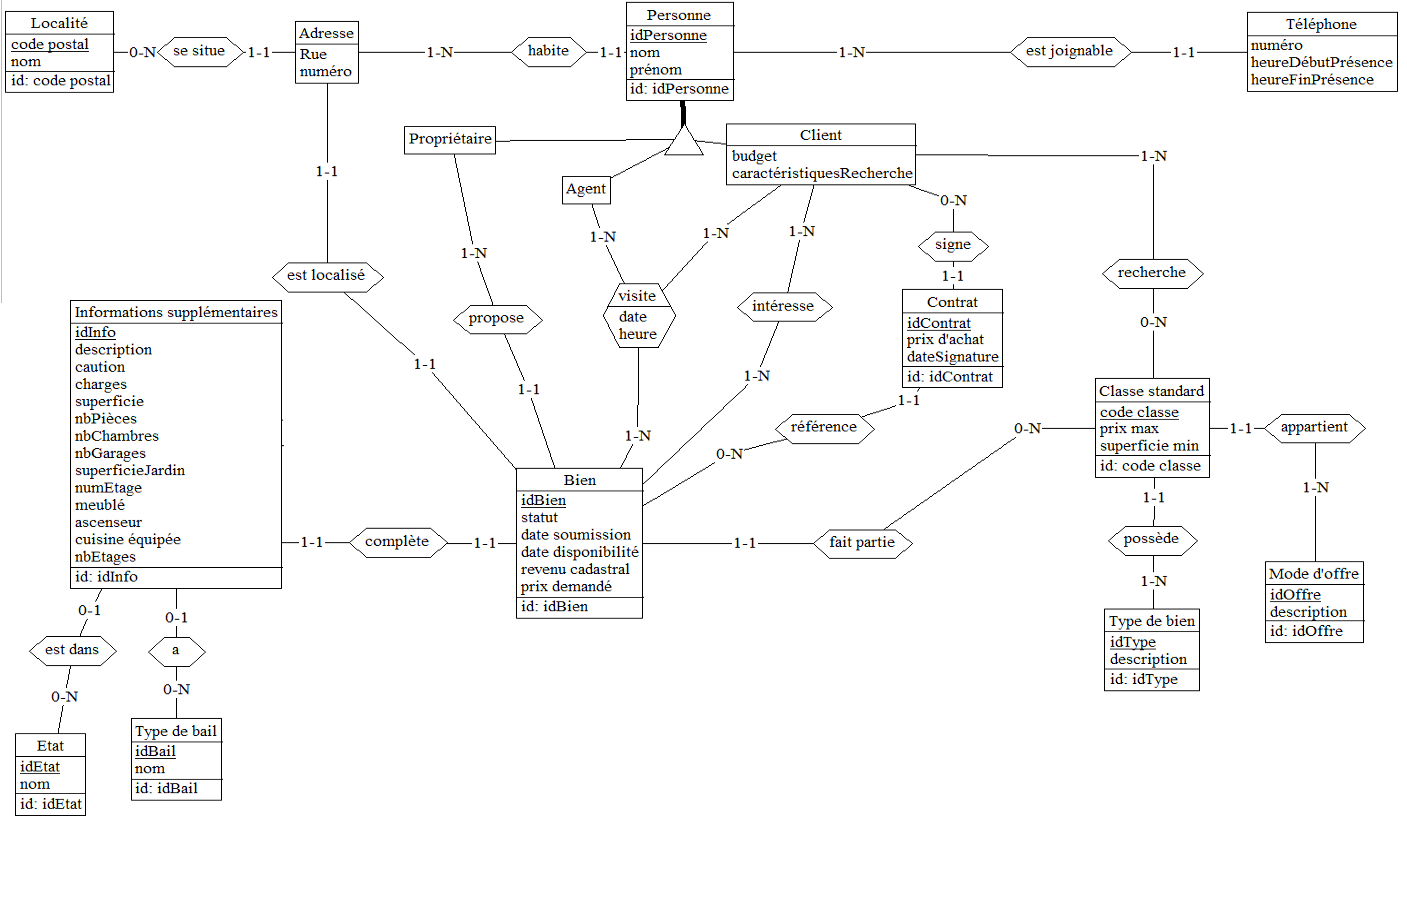
\includegraphics[width=25cm]{association.png}
		\caption{Schéma entité-association final}
		\label{fig:ea}
	\end{figure}
\end{landscape}

\begin{figure}[H]
	\centering
	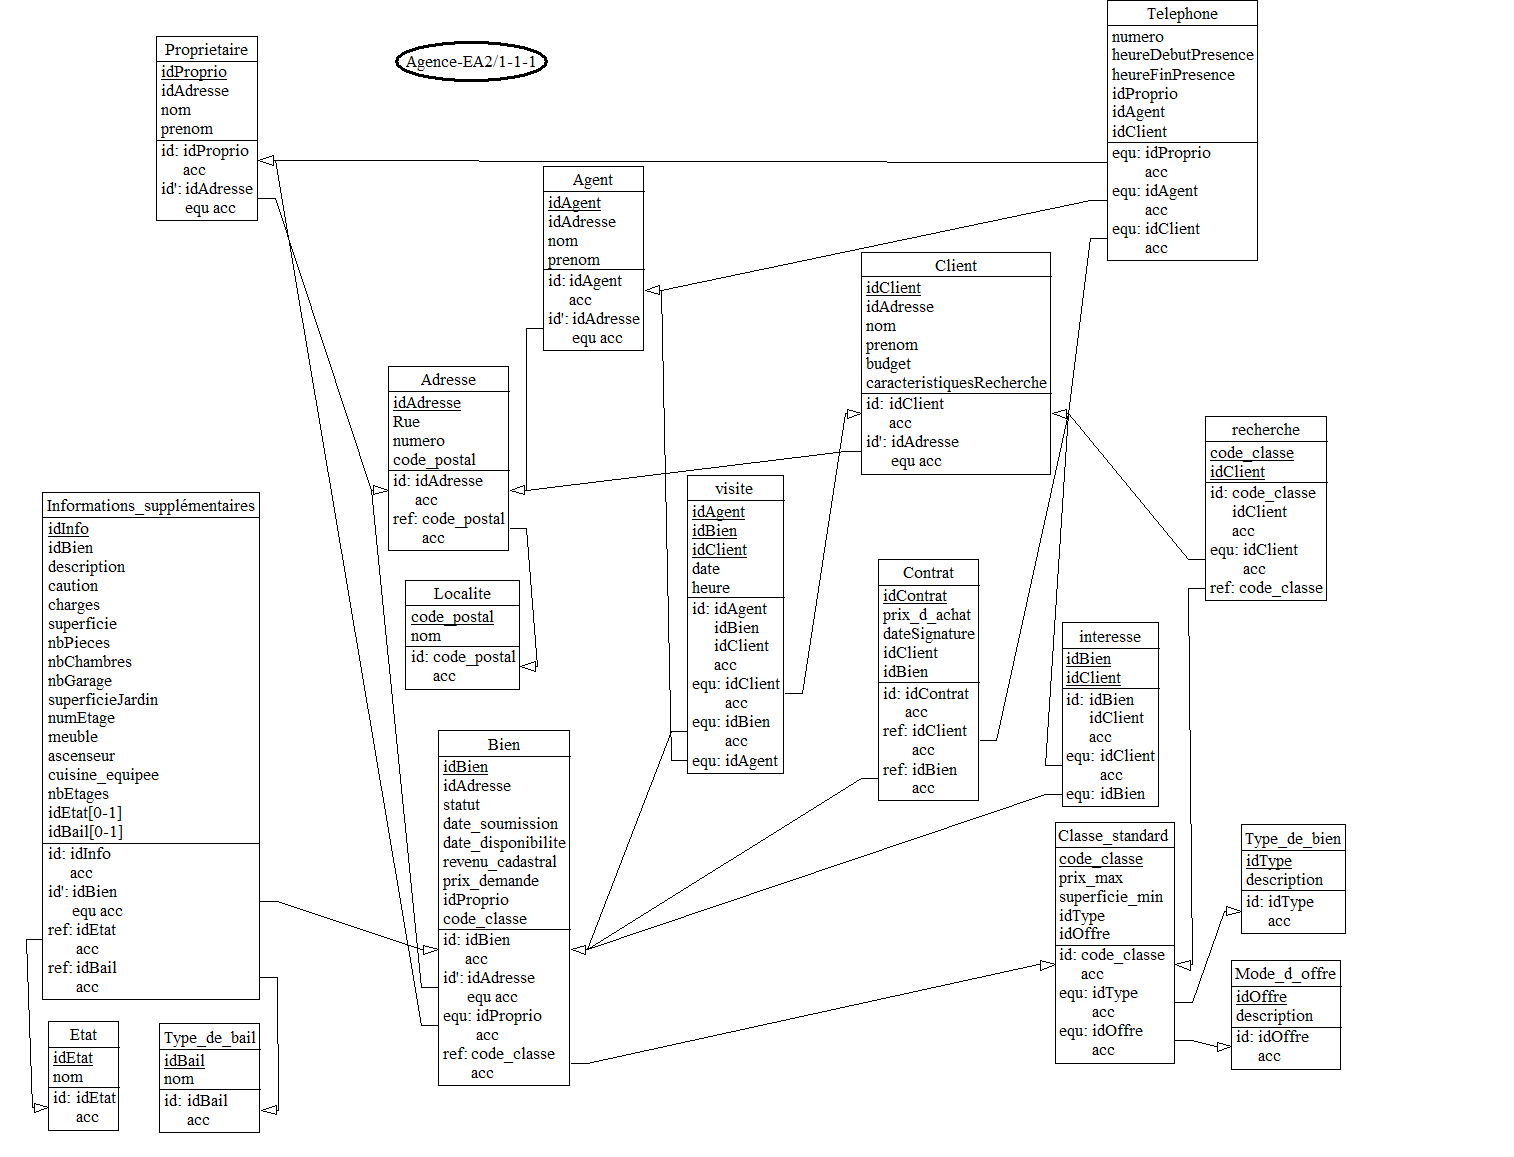
\includegraphics[width=16cm]{relationnel.png}
	\caption{Schéma de la base de données}
	\label{fig:bdd}
\end{figure}

